\documentclass{ctexart}

\usepackage{ctex}
\usepackage{tikz}
\usetikzlibrary{calc,positioning,shapes.geometric}
\usepackage{url}
\usepackage{graphicx}
\usepackage{float}
\usepackage{xcolor}
\usepackage{color}
\usepackage{amsmath}
\usepackage{amsthm}
\usepackage{amssymb}
\usepackage{mathrsfs}
\usepackage{caption}
\usepackage{subfigure}
\usepackage{framed}
\usepackage{booktabs}
\usepackage{makecell}
\usepackage{geometry}
\usepackage{wrapfig}
\usepackage{abstract}
\usepackage{algorithmicx}
\usepackage[ruled]{algorithm}
\usepackage{algpseudocode}
\usepackage{setspace}
\usepackage{bm}
\usepackage{cite}
\usepackage{array}
\usepackage{textcomp}
\usepackage{listings}

\definecolor{shadecolor}{rgb}{0.93,0.93,0.93}
\usepackage{geometry}
\geometry{right=2.5cm,left=2.5cm}

\newtheorem{theorem}{定理}

\pagenumbering{arabic}

\begin{document}
\begin{sloppypar}
\title{\vspace{-3cm} \textbf{Homework 5 of Numerical Analysis}}
\author{刘陈若\;$3200104872$\\信息与计算科学2001}
\date{}

\maketitle

\section*{Theoretical questions}
\subsection*{Problem \uppercase\expandafter{\romannumeral1}}
\begin{proof}[\textbf{Solution.}]
显然,区间$[a,b]$上的连续函数经过求和和数乘运算仍然是$[a,b]$上的连续函数,并且满足加法交换律和数乘的分配律。此外,$f \equiv 0$是加法单位元,$1$是乘法单位元,并且对于任何$[a,b]$上的连续函数$f$,$f+(-f)=0$。由此结合\textbf{Definition B.2}易知$\mathcal{C}[a,b]$是$\mathbb{C}$上的线性空间。

其次,我们证明\textbf{Theorem 5.7}定义的$\left \langle u,v \right \rangle$是该线性空间上的一个内积。对于任意$v \in \mathcal{C}[a,b]$,
\begin{equation}
  \left \langle v,v \right \rangle = \int_a^b \rho (t)|v(t)|^2 \mathrm{d}t \geq 0,
\end{equation}
并且由$\rho(t) > 0, \; |v(t)|^2 \geq 0 $可知$\left \langle v,v \right \rangle = 0$当且仅当$|v(t)|^2 = 0$,即$v = 0$。进一步我们有,
\begin{equation}
    \begin{split}
        &\left \langle u+v,w \right \rangle = \int_a^b \rho(t)[u(t) + v(t)]\overline{w(t)}  \mathrm{d}t = \left \langle u,w \right \rangle + \left \langle v,w \right \rangle, \\
        &\left \langle av,w \right \rangle = \int_a^b a\rho(t)v(t)\overline{w(t)} \mathrm{d}t = a\left \langle v,w \right \rangle, \\
        &\overline{\left \langle w,v \right \rangle} = \overline{\int_a^b \rho(t)w(t)\overline{v(t)} \mathrm{d}t} = \int_a^b \overline{\rho(t)w(t)\overline{v(t)}} \mathrm{d}t = \int_a^b \rho(t)v(t)\overline{w(t)} \mathrm{d}t = \left \langle v,w \right \rangle,
    \end{split}
\end{equation}
其中$u,v,w$是任意$[a,b]$上的连续函数,$a$是任意复数。因此,\textbf{Definition B.108}保证$\left \langle u,v \right \rangle$是该线性空间上的一个内积。

最后,根据等式
\begin{equation}
    \Vert u \Vert_2 = \left(\int_a^b \rho (t)|u(t)|^2 \mathrm{d}t \right)^{\frac{1}{2}} = \sqrt{\left \langle u,u \right \rangle}
\end{equation}
和\textbf{Definition B.113}可知,$\Vert u \Vert_2$是$\mathbb{R}$上的一个范数,从而完成了\textbf{Theorem 5.7}的全部证明。
\end{proof}

\subsection*{Problem \uppercase\expandafter{\romannumeral2}}
\subsubsection*{(a)}
\begin{proof}[\textbf{Solution.}]
只需证明,对于任意不相同的自然数$m,n$都有$\left \langle T_m(x),T_n(x) \right \rangle = 0$。事实上,
\begin{equation}
\begin{split}
    \left \langle T_m(x),T_n(x) \right \rangle &= \int_{-1}^1 \cos(m\arccos x)\cos(n\arccos x)\frac{1}{\sqrt{1-x^2}}  \mathrm{d}x \\
    & = -\int_{-1}^1 \cos(m\arccos x)\cos(n\arccos x) \mathrm{d}(\arccos x) \\
    & = \int_{0}^{\pi} \cos(mt)\cos(nt)\mathrm{d}t \\
    & = \frac{1}{2}\int_{0}^{\pi} \cos[(m+n)t]\mathrm{d}t + \frac{1}{2}\int_{0}^{\pi} \cos[(m-n)t]\mathrm{d}t \\
    & = 0,
\end{split}
\end{equation}
其中最后一步是因为$\sin[(m+n)t]$和$\sin[(m-n)t]$在$t = 0,\pi$时都为0,从而得证。
\end{proof}

\subsubsection*{(b)}
\begin{proof}[\textbf{Solution.}]
当然我们可以直接根据已知的Chebyshev多项式求模长后规范化得到答案,不过此处还是老老实实地仿照\textbf{Example 5.19}进行正交化:
\begin{equation}
    \begin{split}
        &u_1=1,\quad v_1 = u_1 = 1,\quad \Vert v_1 \Vert_2^2 = \int_{-1}^1 \frac{1}{\sqrt{1-x^2}}  \mathrm{d}x= \pi, \quad u_1^* = \frac{1}{\sqrt{\pi}}, \\
        &u_2=x,\quad v_2 = x - \left \langle x,\frac{1}{\sqrt{\pi}} \right \rangle\frac{1}{\sqrt{\pi}} = x,\quad \Vert v_2 \Vert_2^2 = \frac{\pi}{2}  , \quad u_2^* = \sqrt{\frac{2}{\pi}}x, \\
        &u_3=x^2,\quad v_3 = x^2 - \left \langle x^2,\sqrt{\frac{2}{\pi}}x \right \rangle\sqrt{\frac{2}{\pi}}x -  \left \langle x^2,\frac{1}{\sqrt{\pi}} \right \rangle\frac{1}{\sqrt{\pi}} = x^2 - \frac{1}{2},\quad \Vert v_3 \Vert_2^2 = \frac{\pi}{8}  , \quad u_3^* = \sqrt{\frac{8}{\pi}}\left(x^2-\frac{1}{2}\right),
    \end{split}
\end{equation}
至此我们得到了前三个标准化Chebyshev多项式$u_1^*,u_2^*,u_3^*$,其具体表达式如上所示。
\end{proof}

\subsection*{Problem \uppercase\expandafter{\romannumeral3}}
\subsubsection*{(a)}
\begin{proof}[\textbf{Solution.}]
根据上一题的结论,\textbf{Corollary 5.25}以及\textbf{Example 5.28}我们有
\begin{equation}
    \begin{split}
        &b_0 = \left \langle y,u_1^* \right \rangle = \int_{-1}^1 \frac{1}{\sqrt{\pi}}  \mathrm{d}x = \frac{2}{\sqrt{\pi}}, \\
        &b_1 = \left \langle y,u_2^* \right \rangle = \int_{-1}^1 \sqrt{\frac{2}{\pi}}x  \mathrm{d}x = 0, \\
        &b_2 = \left \langle y,u_3^* \right \rangle = \int_{-1}^1 \sqrt{\frac{8}{\pi}}\left(x^2-\frac{1}{2}\right)  \mathrm{d}x = -\sqrt{\frac{8}{9\pi}}.
    \end{split}
\end{equation}
因此,最佳二次多项式近似为$\hat{\varphi} = \frac{2}{\pi} - \frac{8}{3\pi}\left(x^2-\frac{1}{2}\right)=\frac{10}{3\pi} - \frac{8}{3\pi}x^2$。
\end{proof}
\subsubsection*{(b)}
\begin{proof}[\textbf{Solution.}]
根据\textbf{Theorem 5.34}以及\textbf{Example 5.35}我们有
$$
G(1,x,x^2) = 
\begin{bmatrix}
    \left \langle 1,1 \right \rangle & \left \langle 1,x \right \rangle & \left \langle 1,x^2 \right \rangle \\
    \left \langle x,1 \right \rangle & \left \langle x,x \right \rangle & \left \langle x,x^2 \right \rangle\\
    \left \langle x^2,1 \right \rangle& \left \langle x^2,x \right \rangle & \left \langle x^2,x^2 \right \rangle\\
\end{bmatrix}
 = 
\begin{bmatrix}
    \pi & 0 & \frac{\pi}{2} \\
    0 & \frac{\pi}{2} & 0\\
    \frac{\pi}{2} & 0 & \frac{3\pi}{8}\\
\end{bmatrix}
,
$$
$$
\mathbf{c} = 
\begin{bmatrix}
    \left \langle y,1 \right \rangle\\
    \left \langle y,x \right \rangle \\
    \left \langle y,x^2 \right \rangle\\
\end{bmatrix}
 = 
\begin{bmatrix}
    2 \\
    0 \\
    \frac{2}{3} \\
\end{bmatrix}
.
$$
求解方程组$G(1,x,x^2)^T \mathbf{a} = \mathbf{c}$可得,
\begin{equation}
    \mathbf{a} = \left[\frac{10}{3\pi} ,0,- \frac{8}{3\pi}\right]^T.
\end{equation}
因此,最佳二次多项式近似为$\hat{\varphi} = \frac{10}{3\pi} - \frac{8}{3\pi}x^2$。
\end{proof}


\subsection*{Problem \uppercase\expandafter{\romannumeral4}}
\subsubsection*{(a)}
\begin{proof}[\textbf{Solution.}]
和\textbf{Problem \uppercase\expandafter{\romannumeral2}}类似,进行Schimidt正交化过程如下:
\begin{equation}
    \begin{split}
        &u_1=1,\quad v_1 = u_1 = 1,\quad \Vert v_1 \Vert_2^2 = \sum_{i=1}^{12} v_1^2(t_i) = 12, \quad u_1^* = \frac{1}{2\sqrt{3}}, \\
        &u_2=x,\quad v_2 = x - \left \langle x,\frac{1}{2\sqrt{3}}\right \rangle\frac{1}{2\sqrt{3}} = x-\frac{13}{2},\quad \Vert v_2 \Vert_2^2 = 143  , \quad u_2^* = \frac{1}{\sqrt{143}}\left(x-\frac{13}{2}\right), \\
        &u_3=x^2,\quad v_3 = x^2 - \left \langle x^2,\frac{1}{2\sqrt{3}} \right \rangle\frac{1}{2\sqrt{3}} -  \left \langle x^2,\frac{1}{\sqrt{143}}\left(x-\frac{13}{2}\right) \right \rangle\frac{1}{\sqrt{143}}\left(x-\frac{13}{2}\right) = x^2 - 13x+\frac{91}{3}, \\
        &\Vert v_3 \Vert_2^2 = \frac{4004}{3}  , \quad u_3^* = \sqrt{\frac{3}{4004}}\left(x^2 - 13x+\frac{91}{3}\right).
    \end{split}
\end{equation}
至此我们得到了一组正交多项式$u_1^*,u_2^*,u_3^*$,其具体表达式如上所示。
\end{proof}
\subsubsection*{(b)}
\begin{proof}[\textbf{Solution.}]
根据(a)的结论,\textbf{Corollary 5.25}以及\textbf{Example 5.28}我们有
\begin{equation}
    \begin{split}
        &b_0 = \left \langle y,u_1^* \right \rangle = \sum_{i=1}^{12} \frac{1}{2\sqrt{3}}y_i = 277\sqrt{3} , \\
        &b_1 = \left \langle y,u_2^* \right \rangle = \sum_{i=1}^{12} \frac{1}{\sqrt{143}}\left(x_i-\frac{13}{2}\right)y_i = \frac{589}{\sqrt{143}}, \\
        &b_2 = \left \langle y,u_3^* \right \rangle = \sum_{i=1}^{12} \sqrt{\frac{3}{4004}}\left(x_i^2 - 13x_i+\frac{91}{3}\right)y_i = 6034\sqrt{\frac{3}{1001}}.
    \end{split}
\end{equation}
因此,最佳二次多项式近似为
\begin{equation}
    \hat{\varphi} =\frac{277}{2} + \frac{589}{143}\left(x-\frac{13}{2}\right) + \frac{9051}{1001}\left(x^2 - 13x+\frac{91}{3}\right) \approx 9.042x^2 -113.427x + 386.000.
\end{equation}
这和\textbf{Example 5.48}的结论是一致的。
\end{proof}
\subsubsection*{(c)}
\begin{proof}[\textbf{Solution.}]
如果数据集的$x_i\mathrm{’s}$保持不变,但是$y_i\mathrm{’s}$发生变化,从(a)和(b)中很容易可以看出,求解正交多项式$u_1^*,u_2^*,u_3^*$的过程是可以重复利用的,但是计算正交多项式前的系数$b_0,b_1,b_2$的过程是需要重新计算的。

对比正规方程组,可以发现,使用正交多项式进行approximation时,只需要直接更新基前面的系数即可,而正规方程组的更新却涉及到矩阵的运算以及线性方程组的求解。对于大型数据集来说,这可能计算代价高昂。相比之下,正交多项式可以使用简单的公式计算,速度更快,效率更高。
\end{proof}



\section*{Programming assignments}
本次编程作业采用Makefile文件对编译进行统一管理。具体地,在Makefile所在目录下输入\verb|make|
即可完成编译,得到可执行文件\verb|test|。对其运行即可得到各小题的输出结果,具体内容将按问题顺序分别作出说明。需要注意的是,本项目作业使用eigen3进行线性方程组求解,它以\verb|#include <eigen3/Eigen/...>|的形式被调用,因此在编译时需要保持相应的文件关系。
\subsection*{DLS solver.h}
由于作业的头文件并不复杂,此处仅给出一个简单的说明。

\verb|DLS_solver.h|定义了两个类 \verb|DLS_solver| 和 \verb|Normal_equations| 和一个子类 \verb|QR_factorization|。\verb|DLS_solver| 类是一个抽象基类,它定义了一个抽象函数 \verb|solve()|,用来求解最小二乘问题。\verb|Normal_equations| 类继承自 \verb|DLS_solver|,它实现了使用正规方程组来求解最小二乘问题的方法。\verb|QR_factorization| 类继承自 \verb|DLS_solver|,它实现了使用 QR 分解来求解最小二乘问题的方法。这两个类的对象可以接受一个矩阵和一个向量作为输入,它们可以根据这些输入来求解最小二乘问题,并返回解的系数。此外,\verb|Normal_equations| 类还提供了一个函数来返回 Gram 矩阵,而 \verb|QR_factorization| 类提供了一个函数来返回 QR 分解中的 $R$ 矩阵的非零部分$R_1$。
\subsection*{Problem A}
头文件已经实现了使用正规方程组求解最小二乘问题。对于题目中所给的数据,运行程序,输出结果如下:
\begin{shaded}
\begin{verbatim}
The results using normal equations are: 
a0 = 2.17572
a1 = 2.67041
a2 = -0.238444
\end{verbatim}
\end{shaded}
其中$a_0,a_1,a_2$是最佳近似二次多项式$\hat{\varphi} = a_0 + a_1x + a_2x^2$的对应系数。
所有数据点和对应的多项式图像如下所示。
\begin{figure}[H]
\centering
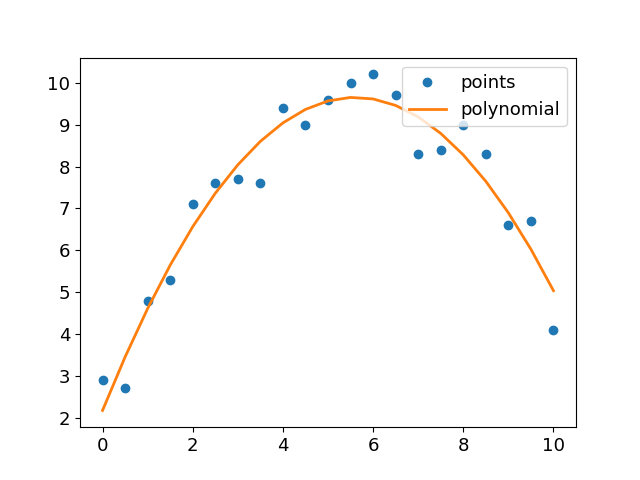
\includegraphics[scale = 0.5]{Figure_1.png}
\label{fig1}
\end{figure}
\subsection*{Problem B}
头文件已经实现了使用QR分解求解最小二乘问题。同时,对于相同的的数据,运行程序,输出结果如下:
\begin{shaded}
\begin{verbatim}
The results using QR factorization are: 
a0 = 2.17572
a1 = 2.67041
a2 = -0.238444
\end{verbatim}
\end{shaded}
其中$a_0,a_1,a_2$是最佳近似二次多项式$\hat{\varphi} = a_0 + a_1x + a_2x^2$的对应系数。可以看出两种不同的算法得到了相同的结果(因此此处不再绘制图像),也从侧面反映了算法的正确和准确性。

进一步,输出正规方程组对应的格拉姆矩阵$G$以及QR分解对应的矩阵$R_1$的条件数如下:
\begin{shaded}
\begin{verbatim}
The condition number of G is: 19002
The condition number of R1 is: 141.072
\end{verbatim}
\end{shaded}
\end{sloppypar}
显然$G$的条件数要远远大于$R_1$的条件数,这也证实了题目所给的结论。
\end{document}
